\documentclass[a4paper,12pt]{article}

\usepackage[ngerman]{babel}
\usepackage[utf8]{inputenc}
\usepackage{amsmath}
\usepackage{amsfonts}
\usepackage{hyperref}
\usepackage{graphicx}
\usepackage{minted}
\usepackage{float}

% http://tex.stackexchange.com/questions/60209/how-to-add-an-extra-level-of-sections-with-headings-below-subsubsection



\begin{document}

% Deckblatt
\begin{titlepage}
\title{Primzahlregression mit Hilfe genetischer Algorithmen}
\author{Björn Boss Henrichsen und Simon Budinsky\\Betreut von Herrn Christoph Fischer}
\date{\today{}}
\maketitle{}
\newpage{}
\end{titlepage}

\tableofcontents{}
\newpage{}


\section{Definitionsverzeichnis}
\subsection{Primzahl}
Eine natürliche Zahl ist genau dann eine Primzahl, wenn sie größer als eins und nur durch sich selbst und eins teilbar ist. Somit ist die Mächtigkeit der Teilermenge einer Primzahl zwei.

\subsection{Effizienz eines Algorithmus}
Ein Algorithmus ist genau dann effizient, wenn er ein vorgegebenes Problem mit möglichst wenig Ressourcenaufwand (zB.: Speicher, Zeit) löst.

\subsection{Laufzeit}
Die Anzhal der Schritte, die ein Algorithmus zur Lösung eines Problems benötigt, wird als Laufzeit bezeichnet.

\subsection{Computercluster}
Ein Computercluster ist Netz aus zusammengeschalteten Computern. Es wird meistens zur Lösung von Problemen verwendet, für die die Leistung eines Computers nicht ausreichend ist.

\newpage{}


\section{Ziel des Projekts}
Bisher gebe es keine Formel, welche Primzahlen effizient berechenbar generiert. 
Wir wollen solch eine mit Hilfe eines genetischen Algorithmus finden. Hierfür soll dieser eine Folge finden, welche möglichst genau Primzahlen beschreibt.

\section{Relevanz von Primzahlen}
Über 2000 Jahre lang konnte man keinen praktischen Nutzen aus dem Wissen über die Primzahlen ziehen. Dies änderte sich erst mit dem Aufkommen elektronischer Rechenmaschinen, bei denen die Primzahlen beispielsweise in der Kryptographie eine zentrale Rolle spielen. So gibt es Verschlüsselungsalgorithmen, welche auf der Primfaktorzerlegung basieren. 
Ein modernes Beispiel hierfür ist der RSA-Algorithmus. Dessen Verschlüsselung ist sicher, da bisher offiziell keine Methode gefunden wurde, Zahlen effizient in ihre Primfaktoren zu zerlegen.

Funktionsweise RSA:
…

Aktuell gibt es einen \href{https://en.wikipedia.org/wiki/RSA_Factoring_Challenge}{RSA-Wettbewerb}. Ziel ist es, die zwei Primfaktoren einer RSA Zahl zu finden. Denn findet man diese, so ist die Verschlüsselung geknackt. Dies wird mit einem entsprechenden Preisgeld belohnt.
Die bisher größte zerlgte RSA Zahl hat 232 Dezimalstellen (768 Bits, RSA-768) und wurde am 12. Dezember 2009 von Thorsten Kleinjung, Paul Zimmermann u.a. für ein Preisgeld von \$ 50000 USD faktorisiert. Hierfür wurde ein Rechencluster verwendet, welches etwa tausend Mal schneller als ein 2,2GHz AMD Opteron single-core Prozessor ist. Trotzdem dauerte die Faktorisierung zwei Jahre. 
Dabei muss bedacht werden, dass heutzutage eher längere RSA-Zahlen verwendet werden. Häufig verbreitet sind Zahlen im Bereich von 309 bis 617 Dezimalstellen (1024-2048 Bits (das Preisgeld für eine RSA-2048-Zahl beträgt aktuell \$ 200000 USD (2.01.17))).
Zusätzlich sollte die Verschlüsselung in ein paar Minuten, am besten wenige Sekunden, erfolgen. So könnte das Passwort zum Bankaccount per Man-In-The-Middle-Angriff einfach ausgelesen werden. Dies ist natürlich nur eine von den vielen fatalen Folgen, wenn RSA geknackt werden würde. Der Mensch könnte seine Privatsphäre verlieren und zum ,,gläsernen Menschen“ werden.
Eine primzahlbeschreibende Folge wird vor allem in der Kryptographie benötigt. Damit RSA funktioniert, werden zunächst zwei Primzahlen erzeugt. Diese müssen zunächst gefunden werden. Hierfür werden Test wie der Rabin-Miller-Test verwendet, der allerdings nur über eine Zahl zwei Aussagen kann: zusammengesetzt oder wahrscheinlich prim. Er liefert also nicht mit hundertprozentiger Sicherheit Zahlen, die anschließend für RSA verwendet werden. Ist eine Zahl nicht prim, funktioniert der RSA-Algorithmus nicht und kann geknackt werden. 
Dies kann verhindert werden, indem stets mit hundertprozentiger Sicherheit über eine Zahl ausgesagt werden kann, ob sie prim ist. Hierfür könnte eine Folge für Primzahlen verwendet werden und somit die Primzahltest ablösen.
Ein weiteres Problem ist folgendes: Finde die nte Primzahl. Beim Sieb des Eratosthenes zum Beispiel müssen zunächst alle Primzahlen vor der nten gefunden werden. Gäbe es eine Folge für Primzahlen, könnte dieses Problem wesentlich effizienter gelöst werden. Folglich wären Algorithmen zum Finden von Primzahlen wie das Sieb des Eratosthenes obsolet.

\newpage{}


\section{Das Sieb des Eratosthenes}
\subsection{Allgemein}
Das Sieb des Eratosthenes ist ein Algorithmus, mit welchen man Primzahlen findet kann. Er wurde
nach dem grieschischen Mathematiker Eratosthenes von Kyrene bennant, welcher im 3. Jahrhundert v. Chr. lebte. Laut \href{https://de.wikipedia.org/wiki/Sieb_des_Eratosthenes}{wikipedia.org} habe dieser selbst nicht das Verfahren entdeckt. Eratosthenes habe lediglich die Bezeichnung ,,Sieb“ eingeführt .
Für Primzahlen kleiner 10000000 zählt der Algorithmus zu den effizientesten Methoden. Für größere Zahlen empfehlen sich effizientere Algorithmen,. Beispiele sind der Lehmann-Test oder der Rabin-Miller-Test, welcher auch in modernen Verschlüsselungsalgortihmen (RSA) verwendet wird.

\subsection{Funktionsweise}
Zu Beginn werden alle natürlichen Zahlen von 2 bis einer Grenze limit aufgeschrieben. Anfangs sind all diese nicht gestrichen und somit potentielle Primzahlen. Nun durchläuft man das Intervall. Trifft man auf eine ungestrichene Zahl, so ist diese eine Primzahl. Jetzt werden alle Vielfachen dieser gestrichen, die größer oder gleich deren Quadrat sind. Ist man am Ende des Intervalls angekommen, liegen sowohl gestrichene als ungestrichene Zahlen vor. Dabei ist jede ungestrichene Zahl prim.

Es genügt, die Vielfachen von Primzahlen zu streichen, die kleiner oder gleich der Wurzel der Grenze limit sind. Denn ist ein Primfaktor einer zusammengesetzten Zahl immer kleiner gleich der Wurzel der zusammengesetzten Zahl.

Außerdem muss beim Streichen der Vielfachen erst mit dem Quadrat der Primzahl begonnen werden, da alle kleineren Vielfachen bereits getrichen wurden.

\newpage{}

\subsection{Offizielle Variante}

\subsubsection{Programmablaufplan}
\begin{figure}[h]
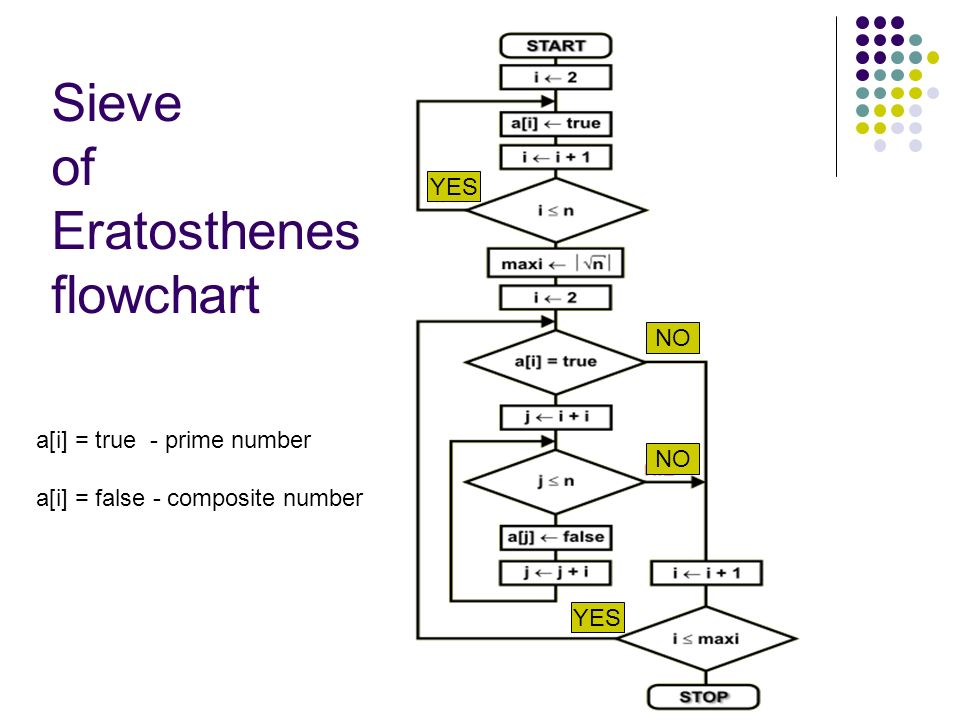
\includegraphics[width=\textwidth]{eratosthenesPAP.jpg}
\end{figure}

\subsubsection{Komplexität}
Die asymptotische Laufzeitkomplexität $O$ in Abhängigkeit von einer oberen Grenze $n$ ergibt sich wie folgt:\\\\
Sei $p_j \in \mathbb{P}$\\
So werden für jede Primzahl 
\[ p_j \leq \sqrt{n} \]
höchstens $\frac{n}{p_j}$ Zahlen gestrichen. Somit erhält man für die Anzahl an ,,Streichungen":\\
\[ \frac{n}{2} + \frac{n}{3} + \frac{n}{5} + ... = \sum_{p_j\leq\sqrt{n}}{\frac{n}{p_j}} = n * \sum_{p_j\leq\sqrt{n}}{\frac{1}{n}}\]
Nun muss die asymptotische Ordnung $o$ vom zweiten Faktor gefunden werden. Diese ist $O$(log log $n$) (Der Beweis hierfür ist nicht trivial und würde den Rahmen der Facharbeit sprengen). Daher ergibt sich eine Gesamtkomplexität von $O$($n$ log log $n$).


\subsection{Optimierungsmaßnamen}

\subsubsection{Weglassen der eins}
Da die eins keine Primzahl ist, kann man sie vorab ignorieren. Somit wird die Länge des primes-Puffers um ein Byte verringert (Speichereffizienz). Zusätzlich muss zu Beginn ein Byte initialisiert werden. In der äußeren for()-Schleife wird ebenfalls ein Durchlauf weniger benötigt (Zeiteffizienz).\\

\subsubsection{Quadrieren statt Radizieren}
Des Weiteren ist das Radizieren an einem Computer ineffizienter als das Quadrieren. Denn kann für das Radizieren eine Bisektion (Software) benötigt werden, wohingegen Quadrieren lediglich eine Multiplikation ist, welche direkt in der ALU (Hardware) ausgeführt werden kann.\\
Somit kann man schreiben:\\
\[ i \leq \sqrt{n} \Rightarrow i * i \leq n \]

\subsubsection{Zahlen im Vorraus streichen}
Der Algorithmus kann weitergehend optimiert werden, indem man Zahlen vorab ,,streicht“. So haben wir alle Vielfachen von zwei bereits ,,gestrichen“. Daraus ergibt sich folgende Speichereinsparung:\\
\\
$a$: Belegter RAM-Speicher mit allen Zahlen\\
$b$: Belegter RAM-Speicher ohne eins und geraden Zahlen\\
$n$: Obere Grenze des Siebes\\
$k$: Proportionalitätsfaktor\\

\begin{align}
a &= k * b\\
\Leftrightarrow n &= k * ( \frac{n}{2} - 1 )\\
\Leftrightarrow k &= \frac{n}{( \frac{n}{2} - 1 )}\\
&= \frac{2n}{n-2}
\end{align}
\\
Foglich verwendet die optimierte Variante $\frac{n-2}{2n}$ Mal so viel Speicher, im Vergleich zur offiziellen. Somit können mehr Primzahlen auf dem gleichen Rechner gefunden werden.\\
\\
Auch zeigen unsere Messungen, dass, wenn man alle Vielfachen von zwei weglässt, der Algorithmus mehr als doppelt so schnell terminiert (Zeiteffizienz).\\
\\
Nach den oben genannten Optimierungen könnte ein Programmablaufplan so aussehen:\\\\
\begin{figure}[H]
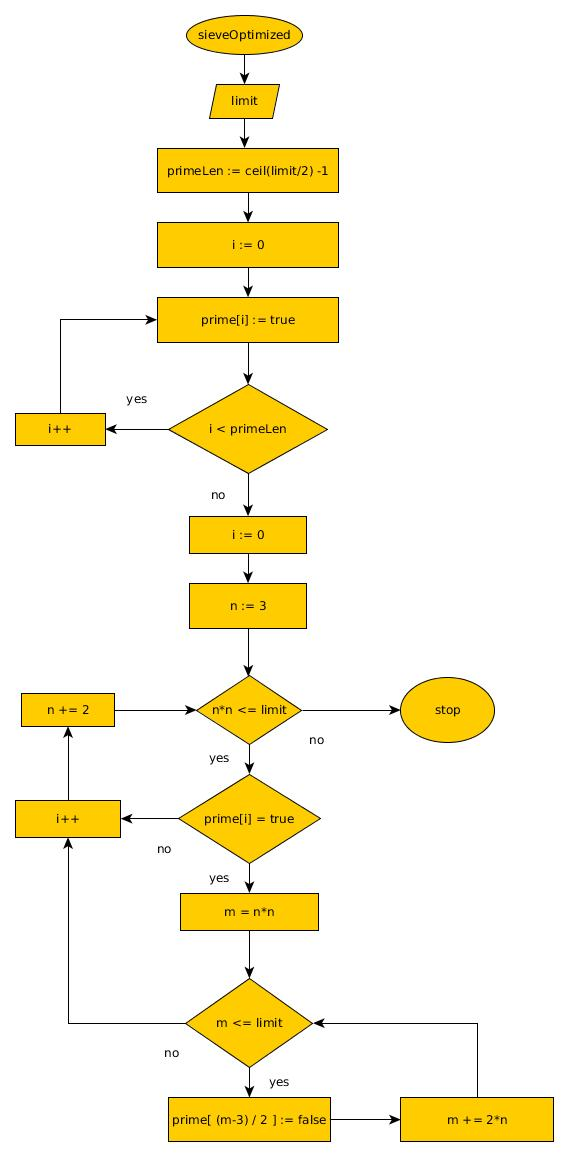
\includegraphics[width=\textwidth,height=\textheight,keepaspectratio]{sieveOptimized.jpg}
\end{figure}

Nun könnte man immer mehr Zahlen im Vorraus ,,streichen". Hierfür gibt es allerdings andere Algortihmen. Der NAME zum Beispeil schließt vorher Zahlen bestimmter Restklassen aus.

\subsection{Messungen}
\subsubsection{Methodik}
Um die Laufzeit des Siebes für verschiedene Grenzen $limit$ zu messen, wurde das Programm für jedes $limit$ jeweils neu kompiliert und ausgeführt. Nachdem die Primzahlen gefunden sind, gibt das Programm die böntigte Zeit zwischen Speicherallokation für den Primzahl-Puffer und dem Finden der Primzahlen in Sekunden aus. Diese Ausgabe wurde in eine .csv-Datei per Linux-Bash umgeleitet, um somit später mit LibreOfficeCalc Diagramme zu erzeugen. Dabei besteht diese Datei aus drei Spalten. Die erste Spalte repräsentiert die aktuelle Grenze $limit$, die zweite die gemessene Zeit in Sekunden und in der dritten Spalte steht die Anzahl gefundener Primzahlen.
\\\\
Dafür verwendeten wir folgendes Bash-Script:

\begin{minted}[frame=lines]{bash}
#!/bin/bash
#i: limit
for i in {100000000..6000000000..100000000}
do
    echo -n "$i," >> runtimes.csv
    gcc -std=c11 -DLIMIT=$i sieveRuntime.c -o sieveRuntime -lm \
		&& ./sieveRuntime >> runtimes.csv
done
\end{minted}

Wir implementierten folgende Algorithmen in C zur Zeitmessung:\\
Sieb ohne die eins:\\\\
\begin{minted}[frame=lines]{C}
#include    <inttypes.h>
#include    <stdbool.h>
#include    <stdlib.h>
#include    <string.h>
#include    <sys/time.h>
#include    <stdio.h>


int main( void ) {
    struct timeval  start, end;
    gettimeofday(&start, NULL);
    
    bool* prime = (bool*)malloc(sizeof(bool) * (LIMIT-1));
    if( prime == NULL ) return 1;


    memset(prime, true, LIMIT-1);

    for(uint64_t i = 2; i*i <= LIMIT; i++) {
        if(prime[i-2]) {

            for(uint64_t j = i*i -2; j <= LIMIT; j += i) {
                prime[j] = false;
            }
        }
	}


    gettimeofday(&end, NULL);
    
    // Count primes
    uint32_t    nPrimes  = 0;
    for( uint32_t i = 0;  i < LIMIT-1; i++) {
        if( prime[i] ) nPrimes++;
    }   
    
    printf("%.10f,%" PRIu32 "\n", 
	 end.tv_sec + end.tv_usec/1e6 - start.tv_sec - start.tv_usec/1e6, 
	  nPrimes);
    
	return 0;
}
\end{minted}

Sieb ohne die eins und geraden Zahlen:\\\\
\begin{minted}[frame=lines]{C}
#include    <inttypes.h>
#include    <stdbool.h>
#include    <stdlib.h>
#include    <string.h>
#include    <sys/time.h>
#include    <stdio.h>
#include    <math.h>


int main( void ) {
    struct timeval  start, end;
    gettimeofday(&start, NULL);

    uint32_t	primeLen = ceil(LIMIT / 2) - 1;
    bool* 		prime 	 = (bool*)malloc(sizeof(bool) * primeLen);
    if( prime == NULL ) return 1;

    memset(prime, true, primeLen);


    for(uint64_t i = 0, n = 3;  n*n <= LIMIT;  i++, n += 2) {
        if(prime[i]) {


            for(uint64_t m = n*n;  m <= LIMIT;  m += 2*n) {
				prime[ (m-3) / 2 ] = false;
            }
        }
	}


    gettimeofday(&end, NULL);
    
    // Count primes
    uint32_t    nPrimes  = 1;
    for( uint32_t i = 0;  i < primeLen; i++) {
        if( prime[i] ) nPrimes++;
    }   
    
    printf("%.10f,%" PRIu32 "\n", 
     end.tv_sec + end.tv_usec/1e6 - start.tv_sec - start.tv_usec/1e6, 
      nPrimes);
    
	return 0;
}
\end{minted}

Anmerkung:\\
Es wird bewusst nicht die Zeit zum Ausgeben (printf()) mit einbezogen, da diese allgemein einen großen Anteil an Laufzeit beansprucht. Vergleicht man die folgenden Messwerte, so ergibt sich bei unserem optimierten Algorithmus für n = 1.000.000 eine Zeit von etwa 1389.054 Sekunden mit Ausgabe aller Primzahlen und etwa 8.0484920487 Sekunden ohne.

Die Messungen fanden in folgender Umgebung statt:\\\\
\begin{tabular}{|r|l|}
\hline
Operating System & \emph{Linux Mint 18.1 Cinnamon 64-Bit}\\
Cinnamon Version & \emph{3.2.7}\\
Linux Kernel & \emph{4.4.0-53-generic}\\
Processor & \emph{Intel Core i5-4440 CPU @ 3.10GHz x 4}\\
Memory RAM & \emph{7.7GiB}\\
\hline
\end{tabular}\\\\

\subsubsection{Vergleich zwischen offizieller und optimierter Variante}
$t_g$: Benötigte Zeit in Sekunden, offizielle Variante (blau)\\
$t_u$: Benötigte Zeit in Sekunden, optimierte Variante (rot)\\
\begin{tabular}{|c|c|c|c|}
\hline
$limit$ & $t_g$[s] & $t_u$[s] & $\frac{t_g}{t_u}$\\
\hline
100000000 & 1,6142570771 & 0,6927529358 & 2,3302060427\\
200000000 & 3,3796610065 & 1,5407490117 & 2,193518205\\
300000000 & 5,2564000593 & 2,2783710453 & 2,3070869296\\
400000000 & 6,7034089816 & 3,1714290402 & 2,1136872043\\
500000000 & 8,9381100896 & 3,9901179841 & 2,2400616035\\
600000000 & 10,3455499889 & 5,011878017 & 2,0642062624\\
700000000 & 12,6841129465 & 5,5832778916 & 2,271803982\\
800000000 & 13,9744109066 & 6,8093409411 & 2,0522413296\\
900000000 & 15,8358931078 & 7,3026679844 & 2,1685078853\\
1000000000 & 18,0069118877 & 8,0484920487 & 2,2373025629\\
1100000000 & 19,4879198822 & 9,4263940965 & 2,0673780114\\
1200000000 & 22,4203640433 & 10,0174689825 & 2,2381266248\\
1300000000 & 23,5954410898 & 10,3775840185 & 2,2736930915\\
1400000000 & 26,5114490883 & 11,0751651153 & 2,393774613\\
1500000000 & 26,9755919041 & 11,9925879208 & 2,2493553587\\
1600000000 & 30,2582220339 & 13,9449501191 & 2,1698336513\\
1700000000 & 32,2235829942 & 14,2521269333 & 2,2609666013\\
1800000000 & 32,8872118869 & 14,924550968 & 2,2035645801\\
1900000000 & 36,7206629502 & 16,3945279494 & 2,2398121534\\
2000000000 & 38,3611690887 & 16,617560026 & 2,3084718231\\
2100000000 & 39,3934800971 & 17,4123429244 & 2,2623882534\\
2200000000 & 42,4355878925 & 19,252283056 & 2,2041847073\\
2300000000 & 43,353328041 & 20,0979319791 & 2,1571039292\\
2400000000 & 45,0081739355 & 20,6734950301 & 2,1770955453\\
2500000000 & 49,1815101048 & 22,0877529756 & 2,2266416217\\
2600000000 & 51,3432890466 & 22,012063034 & 2,3325069062\\
2700000000 & 51,1586249138 & 24,0191830281 & 2,129906952\\
2800000000 & 53,3409920051 & 24,7522308979 & 2,1549973505\\
2900000000 & 55,47018401 & 24,3075119497 & 2,282018173\\
3000000000 & 56,9847639827 & 26,5199970692 & 2,148746994\\
3100000000 & 60,5142700262 & 27,7222269376 & 2,1828791086\\
3200000000 & 60,012045889 & 28,7487220151 & 2,0874683006\\
3300000000 & 65,3936210892 & 29,68840601 & 2,2026652784\\
3400000000 & 62,9704729115 & 29,7541698854 & 2,116357914\\
3500000000 & 69,8409569373 & 31,0977290192 & 2,2458539302\\
3600000000 & 67,1172831177 & 30,4034039054 & 2,2075581842\\
3700000000 & 73,4939509822 & 32,2375419811 & 2,2797628624\\
3800000000 & 76,0375679339 & 31,9458291063 & 2,3802033023\\
3900000000 & 78,455664996 & 33,7550660629 & 2,3242634113\\
4000000000 & 80,9324689933 & 35,4401829989 & 2,2836357531\\
4100000000 & 82,0384289596 & 37,5744409737 & 2,1833572725\\
4200000000 & 79,314230075 & 36,3971849106 & 2,1791308935\\
\hline
\end{tabular}

\begin{figure}
\includegraphics[width=\textwidth]{comparison.png}
\end{figure}


\subsubsection{Messung mit Ausgabe aller Primzahlen}
\begin{tabular}{|c|c|c|c|c|}
\hline
$limit$ & $t_g$[s] & $t_u$[s] & $\Delta t$ & $anzahl$ \\
\hline
100.000 & 0,003 & 0,002 & 0,001 & 9592\\
1.000.000 & 1,216 & 1,205 & 0,011 & 78498\\
10.000.000 & 14,463 & 14,387 & 0,076 & 664579\\
100.000.000 & 143,18 & 142,439 & 0,741 & 5761455\\
1.000.000.000 & 1397,5 & 1389,054 & 8,446 & 50847534\\
\hline
\end{tabular}


%\newpage{}
%\subsubsection{Programmablaufplan}
%\begin{figure}[h]
%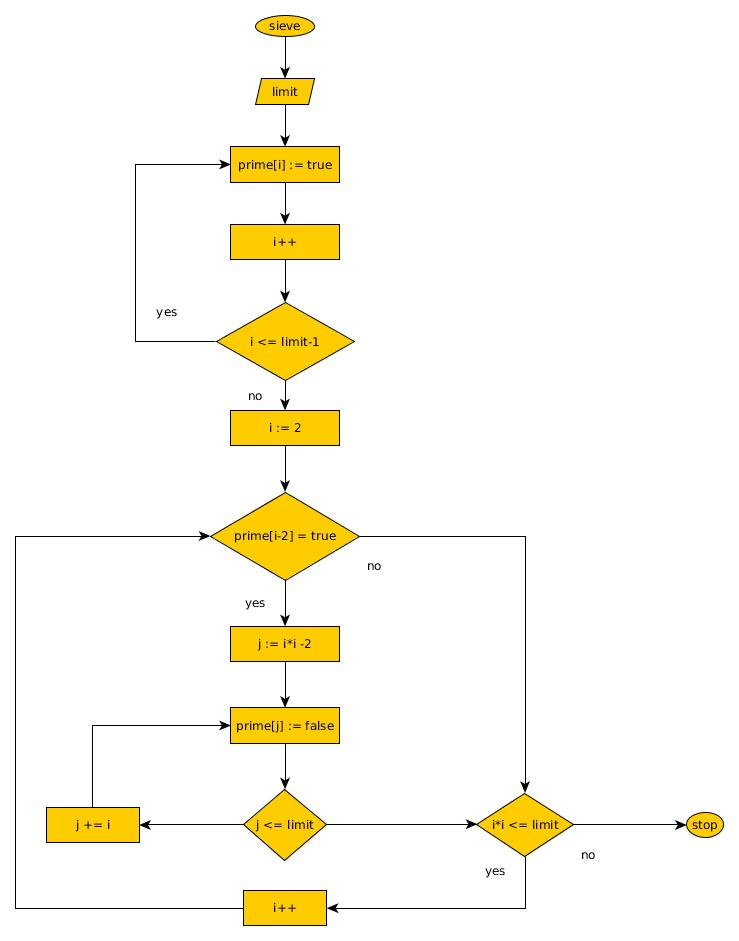
\includegraphics[width=\textwidth]{sieve.jpg}
%\end{figure}




\end{document}
